\documentclass[]{article}
\usepackage{amsmath}\usepackage{amsfonts}
\usepackage[margin=1in,footskip=0.25in]{geometry}
\usepackage{mathtools}
\usepackage{hyperref}
\hypersetup{
    colorlinks=true,
    linkcolor=blue,
    filecolor=magenta,
    urlcolor=cyan,
}
\usepackage[final]{graphicx}
\usepackage{listings}
\usepackage{courier}
\lstset{basicstyle=\footnotesize\ttfamily,breaklines=true}

% \usepackage{wrapfig}
\graphicspath{{.}}
\begin{document}

\begin{center}
    CSE 546 SPRING 2021: HW1 
\end{center}
\begin{center}
    Name: Honda Li
\end{center}

\section*{Short Answer and ``True or False'' Conceptual Questions}
    \subsection*{A.0}
        \subsubsection*{A.0.a}
            The bias and variance is similar to the concepts of precision and accuracy in Experimental Physics. Under the context of machine learning, Bias refers to part of the learning errors caused by a model being too simple, in a way that it just cant represent the joint probability density function with its simplicity. 
            \\[1em]
            The variance refers to the variance of the random variable $\hat{f}(x)$, which depends on the samples we observed. 
            \\[1em]
            Bias-variance trade off relates 2 types of learning errors (Bias, Variance) with the model complexity. 
        \subsubsection*{A.0.b}
            Usually, higher the model complexity, higher the variance, lower the model complexity, higher the bias. 
        \subsubsection*{A.0.c}
            False. The bias decreases. Because the bias is: $\mathbb{E}\left[
                \left(
                f(x) - \mathbb{E}\left[\hat{f}(x)\right]
                \right)^2
            \right]$. The number of sample seems to be irrelevant to the amount of bias we have for the model. 
        \subsubsection*{A.0.d}
            True, the model variance decreases as the number of samples increases, when the model complexity is a fixed quantity.  
            \\
            The best model is the model that: Minimizes the square loss function of the joint expectation: $\mathbb{E}_{Y|X}\left[(Y - \eta{X})^2\right]$, and notice that because of the square loss function, the solution to the problem is unqiue. And because we are increasing the number of sample to infinite, we approximate the true distribution (the populations) better and better. Therefore, the best estimated model must converge, which means that the variance will decrease. 
        \subsubsection*{A.0.e}
            Yes, and this is exactly the idea behind regularization, where it tries to change the objective of the optimization problem a bit, allowing the models to use less features and prevent it from over-fitting. This improves the ability for the model to generaize better by reduce the model variance of the model. 
        \subsubsection*{A.0.f}
            We should use the train set to tune the hyper-parameters for the models. This is true because the test set is for the final benchmark for our models. 
            \\
            Consider polynomial regression, we can use cross validations (Which only uses the training set) to look for the models with the least amount of variance, or models with the least amount of error or something in between them. 
        \subsubsection*{A.0.g}
            False. It's an underestimate, which is a conclusion from the lecture.

\section*{Maximum Likelihood Estimator(MLE)}
    \subsection*{A.1}
        \subsubsection*{(A.1.a)}\label{A.1.a}
            \textbf{Objective}: Find the expression for the maximum=likelihood estimate for the parameter $\lambda$ for the poisson distribution, interns of the goal count. Assume idd rvs. 
            \\[1em]
            Here we will assume that observations obtained takes the form $x_1, x_2, \cdots x_N$, and then we derive the best estimator for $\lambda$ in this much general context. 
            \\[1em]
            I will shut up and just show you the math: 
            \begin{align*}\tag{A.1.a.1}\label{eqn:A.1.a.1}
                & 
                \prod_{n = 1}^{N} 
                \text{Poi}(x_n|\lambda)
                \\
                &
                \sum_{n = 1}^{N}
                \log\left(
                    \text{Poi}(x_n|\lambda)
                \right)
                \\
                &
                \sum_{n = 1}^{N}
                \left(
                    -\lambda + x_n\ln(\lambda) + \log(x_n!)
                \right)
            \end{align*}
            Notice that, only some of the terms are relevant to the parameter $\lambda$, therefore, the optimization problem we are solving is: 
            \begin{equation*}\tag{A.1.a.2}\label{eqn:A.1.a.2}
                \lambda^+ = 
                \underset{\lambda}{\text{argmax}}
                \left\lbrace
                    -N\lambda
                    +  
                    \ln(\lambda)
                    \sum_{i = 1}^{N}
                        \left(
                            x_n
                        \right)
                \right\rbrace
            \end{equation*}
            To solve it, we just take the derivative, set it to zero and then solve for $\lambda$, because this function is a function that has a single local maximum. 
            \begin{align*}\tag{A.1.a.3}\label{eqn:A.1.a.3}
                \partial_\lambda \left[
                -N\lambda
                +  
                \ln(\lambda)
                \sum_{i = 1}^{N}
                    \left(
                        x_n
                    \right)
                \right] =& 0
                \\
                -N + \frac{\sum_{n = 1}^{N}x_n}{
                \lambda^+
                } =& 0 
                \\
                \implies
                \lambda^+ =& \frac{\sum_{n = 1}^{N}x_n}{N}
            \end{align*}
            Therefor, for this particular problem, the best estimator will be the average of all the observation, which is just: 
            $$
                \frac{2 + 4 + 6 + 1}{5} = 2.6
            $$
            And that is the answer for the question. 
        \subsubsection*{(A.1.b)}\label{A.1.b}
            The derivation of the best estimator in the general context is shown in \hyperref[A.1.a]{A.1.a}. 
            \\[1em]
            The numerical value for six observations is: 
            $$
                \frac{2 + 4 + 6 + 1 + 3}{7} = 2.6666666666\cdots
            $$
        \subsubsection*{(A.1.c)}
            The numerical results for 5 observations has been shown in \hyperref[A.1.a]{A.1.a} and \hyperref[A.1.b]{A.1.b} respectively. 
            
    \subsection*{A.2}
        \textbf{Objective: } Find the MLE for the uniform distribution on $[o, \theta]$, where $\theta$ is the value we want to estimate.
        \\[1em]
        Suppose that observations has been made: $x_1, x_2, \cdots x_N$, and we assume that they are idd, and we want to find the likelihood of such an observation is generated using the Uniform distribution. And this will be given by the expression: 
        \begin{equation*}\tag{A.2.1}\label{eqn:A.2.1}
            \prod_{n = 1}^{N} 
            \underbrace{
            \mathbb{P}\left(X = x_n\right)}_{\frac{1}{\theta}\mathbf{1}\{0 \le x_n \le \theta\}}
        \end{equation*}
        \\[1em]
        Observe that, if any of the observation is beyond the range $[0, \theta]$, we will have zero likelihood, so let's assume that $\theta \ge \max_{1\le i \le N}(x_i)$, then we will have this expression for the likelihood: 
        \begin{equation*}\tag{A.2.2}\label{eqn:A.2.2}
            \prod_{n = 1}^{N} 
            \frac{1}{\theta} = \frac{1}{\theta^N}
        \end{equation*}
        And taking the log on that we have: 
        \begin{equation*}\tag{A.2.3}\label{eqn:A.2.3}
            \log\left(\frac{1}{\theta^N}\right) = -N\log(\theta)
        \end{equation*}
        \\[1em]
        Observe that that function is monotonically decreasing as the value of $\theta$ get larger and larger, therefore, to maximize the likelihood, we need the value of $\theta$ to be as small as possible, and the smallest possible such $\theta$ that is not giving us zero likelihood is: $\max_{1\le i \le N}(x_i)$, therefore, best estimate is given by: 
        $$
            \theta^+ =\max_{1\le i \le N}(x_i)
        $$

\section*{Over-fitting}
    \subsection*{A.3}
        \begin{enumerate}
        \item[1.] $S = \{(x_i, y_i)\}_{i = 1}^N$ drawn from idd with underlying joint distribution $\mathcal{D}$. 
        \item[2.] The training set is break into $S_\text{train}, S_\text{test}$, and $S = S_\text{Train} \cup S_\text{Test}$, notice that overlapping is possible. 
        \item[3.] And the true least square error, given a predictive model $f$ is: $\epsilon(f) = \mathbb{E}\left[(f(x) d - y)^2\right]$. 
        \end{enumerate}
    \subsubsection*{A.3.a}
        We want to show that that, the expected bias of the model $f$ over the training set and the test set is the same as expected value of the bias over the distribution $\mathcal{D}$, hence it's unbiased. 
        \\[1em]
        Start by considering the expected value of $\epsilon_\text{train}(f)$: 
        \begin{align*}\tag{A.3.a.1}\label{eqn:A.3.a.1}
            & \mathbb{E}_{\text{train}}\left[\frac{1}{N_\text{train}}
            \sum_{(x, y)\in S_\text{train}}^{}\left(
                f(x) - y
            \right)^2\right]
            \\
            = &
            \frac{1}{N_\text{train}} 
            \sum_{(x, y)\in S_\text{train}}^{}
            \underbrace{
                \mathbb{E}_{\text{train}}
                \left[ 
                \left(
                    f(x) - y
                \right)^2\right]
            }_{\epsilon(f)}
            \\
            \hat{\epsilon}(f)
            = &
            \hat{\epsilon}_{\text{train}}(f)
        \end{align*}
        For each term $f(x) - y$, we assume that it's idd, and therefore, its expected value is going to be the same as if it's drawn from the distribution $\mathcal{D}$, because each sample of the train set is drawn in this way, therefore, we can conclude that $\mathbb{E}\left[(f(x) - y)^2\right]$ is going to give $\epsilon(f)$. 
        \\[1em]
        The proof for $\hat{\epsilon}_\text{test}(f)$ is going to be exact same because they are both drawn from the same idd joint distribution: $\mathcal{D}$. And hence we know that the bias estimator for any given model is going to be unbiased. Since both has the same variance we know that: 
        \begin{equation*}\tag{A.3.a.2}\label{eqn:A.3.a.2}
            \mathbb{E}_\text{train}\left[\hat{\epsilon}_\text{train}(f)\right]
            =
            \mathbb{E}_\text{test}\left[\hat{\epsilon}_\text{test}(f)\right]
            =
            \hat{\epsilon}(f) 
        \end{equation*}
    \subsubsection*{A.3.b}
        $\mathbb{E}_{\text{train}}\left[\hat{\epsilon}_\text{train}(\hat{f})\right]\ne \epsilon(\hat{f})$ Consider Linear regression where the sample size is so small ($d + 1$ samples where $d$ is the number of features) that we have a perfect fit model $\hat{f}$ then the bias of the model is going to be zero under the training set, however, the bias over the real distribution is not, because $\mathcal{D}$ could be non-linear and there could be noises, which both will introduce some biased. 
    \subsubsection*{A.3.c}
        Some explanations are needed for this question. Consider the following expression: 
        \begin{equation*}\tag{A.3.c.1.1}\label{eqn:A.3.c.1.1}
            \mathbb{E}_\text{train} 
            \left[\hat{\epsilon}_\text{train}(\hat{f}_\text{train})\right]
            \le
            \mathbb{E}_{\text{train, test }}\left[
                \hat{\epsilon}_\text{test}
                (\hat{f}_\text{train})
            \right]
        \end{equation*}
        This is saying that, the expected value of the error on trained estimator evaluated using the test samples by enumerating over all the test samples is less than The expected value of the error when we train the model with train set and get the error with the test set. 
        The estimator of the model is obtained via the following procedures: 
        \\[1em]
        Let $\mathcal{F} = \{f_1, f_2\cdots\}$ be a collection of functions and $\hat{f}$ will minimizes the error given the training set. Now let's consider the error the expected value of the error on the test set of the estimator obtained from the train set: 
        \begin{align*}\tag{A.3.c.2}\label{eqn:A.3.c.2}
            \mathbb{E}_{\text{train, test }}\left[
                \hat{\epsilon}_\text{test}
                (\hat{f}_\text{train})
            \right]\beta
            = &
            \sum_{f\in\mathcal{F}}^{}\mathbb{E}_\text{train, test}
            \left[
                \hat{\epsilon}_{\text{\text{test}}}(f)\mathbf{1}\{\hat{f}_\text{train} = f\}
            \right]
            \\
            \underset{\text{(1)}}{=} &
            \sum_{f\in\mathcal{F}}^{}
            \mathbb{E}_\text{test}\left[
                \hat{\epsilon}(f)
            \right]
            \mathbb{E}_\text{train}\left[\epsilon_\text{test}
                \mathbf{1}\{\hat{f}_\text{train} = f\}
            \right]
            \\
            = &
            \sum_{f\in\mathcal{F}}^{}
            \mathbb{E}_\text{test}\left[
                \hat{\epsilon}_\text{test}(f)
            \right]
            \mathbb{P}\left(
                \hat{f}_\text{train} = f
            \right)
            \\
            = &
            \mathbb{E}_\text{test}\left[
                \hat{\epsilon}_\text{test}(f)
            \right]
            \\
            \underset{\text{(2)}}{=}&
            \mathbb{E}_\text{train}\left[
                \hat{\epsilon}_\text{train}(f)
            \right]
        \end{align*}
        (1) This is by the independence between the test and the training set, therefore, 2 random variable based on each one them can have the expected value operator distributes over. (2) this is by results from \hyperref[eqn:A.3.a.2]{A.3.a.2}. Now, by the definition that $\hat{f}$ minimizes the error compare to all other models on the training setm then by definition, the expected value of it is going to keep the inequality, therefore: 
        \begin{align*}\tag{A.3.c.1}\label{eqn:A.3.c.1}
            & \hat{f} = \min_{f\in\mathcal{F}} \hat{\epsilon}_\text{train}(f)
            \\
            \implies & 
            \mathbb{E}_\text{train} 
            \left[\hat{\epsilon}_\text{train}(\hat{f}_\text{train})\right]
            \le 
            \mathbb{E}_\text{train}\left[
                \hat{\epsilon}_\text{train}(f)
            \right]
            =
            \mathbb{E}_{\text{train, test }}\left[
                \hat{\epsilon}_\text{test}
                (\hat{f}_\text{train})
            \right]
        \end{align*}
        And this is what we want to show for this problem. 
\section*{Polynomial Regression}
    \section*{A.4}
        This part is too simple. See \hyperref[lst:A.5.1]{A.5.1}
    \section*{A.5}
        Code has been implemented. Here is the procedures for fitting the models: 
        \begin{enumerate}
        \item[1.] Augmenting the features by raising the features to it's polynomials powers. Here we assume that the feature sare not interaction. Stack the initial feature columns horizontally to produce the Vandermonde matrix for the features. 
        \item[2.] Standardizing the data across the features (the columns) by it's standard deviation. This is just deviding each column by the sd of that column  
        \item[3.] Adding an additional rows of ones. 
        \item[4.] Creating the regularizer as a diagonal matrix, but the bottom right corner of the diagonal matrix is seet to zeero so we don't regularize on the offset for the regression model.  
        \end{enumerate}
        \label{lst:A.5.1}
        \textbf{NOTE}: for sample size less than 3, I ignore it and didn't override the error np.array that is given. I did this to get the correct scaling on the graph so it looks exactly the same as the graph given by the HW sheet, and I indeed got a graph that looks like what is given non the hW sheet.
        \\
        And the graph I got is exactly the same as same as the HW sheet. 
        \begin{center}
            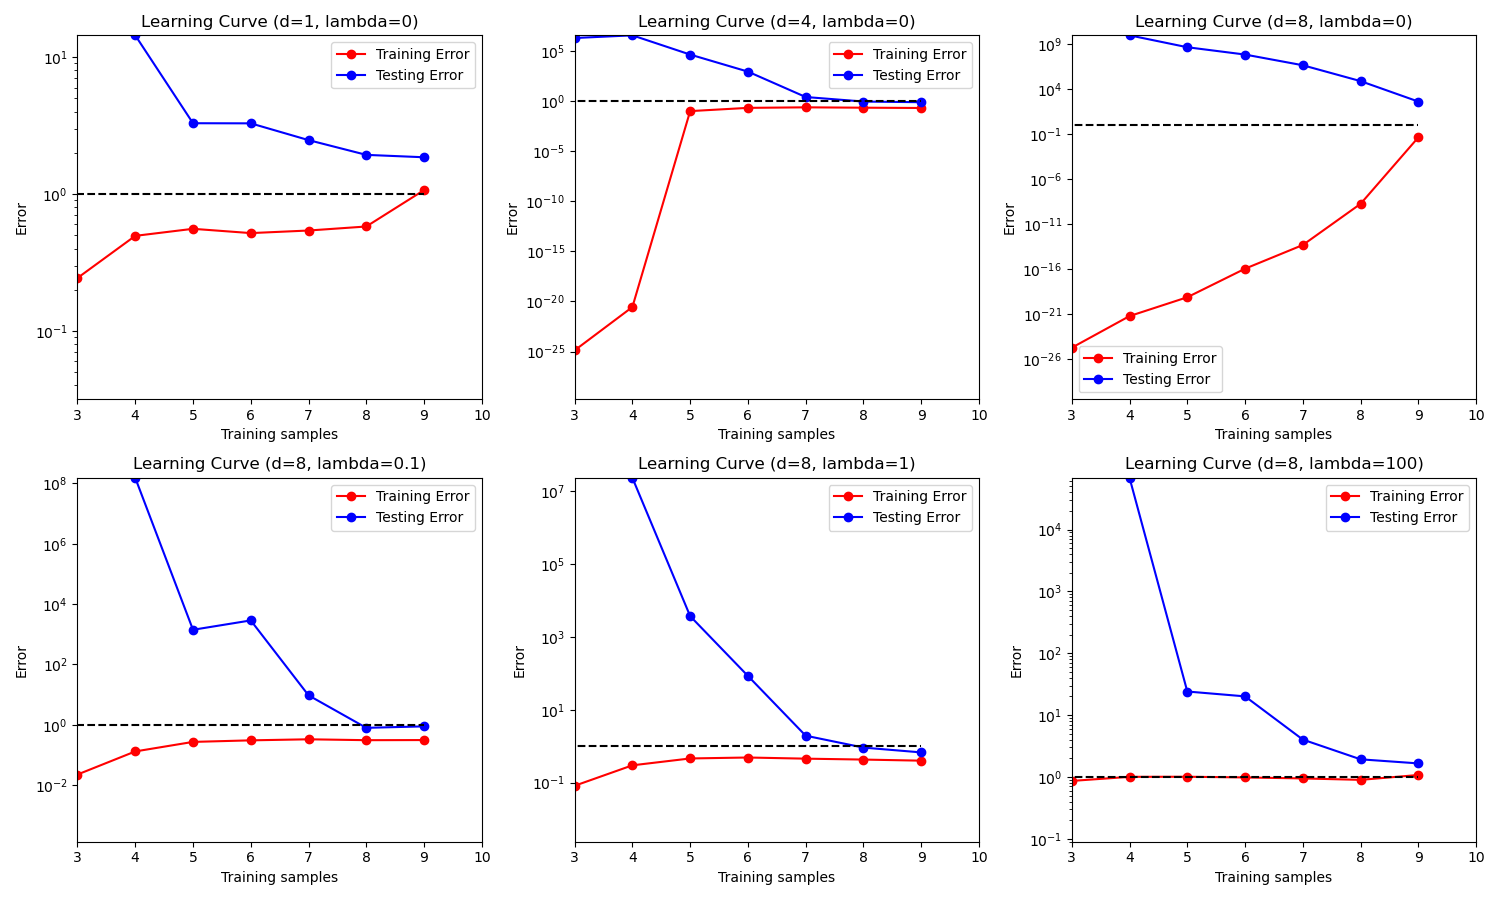
\includegraphics[width=10cm]{myplot.png}    
        \end{center}
        \begin{lstlisting}[language=python]
'''
    Template for polynomial regression
    AUTHOR Eric Eaton, Xiaoxiang Hu
'''

import numpy as np


#-----------------------------------------------------------------
#  Class PolynomialRegression
#-----------------------------------------------------------------

class PolynomialRegression:

    def __init__(this, degree=1, reg_lambda=1E-8):
        """
        Constructor
        """
        this.Degree = degree
        this.Lambda = reg_lambda


    def polyfeatures(self, X, degree):
        """
        Expands the given X into an n * d array of polynomial features of
            degree d.

        Returns:
            A n-by-d numpy array, with each row comprising of
            X, X * X, X ** 3, ... up to the dth power of X.
            Note that the returned matrix will not include the zero-th power.

        Arguments:
            X is an n-by-1 column numpy array
            degree is a positive integer
        """
        assert len(X.shape) == 2 and X.shape[1] == 1, "Wrong input shape for X for polyfeatures."
        return np.hstack([X**II for II in range(1, degree + 1)])


    def fit(this, X, y):
        """
            Trains the model
            Arguments:
                X is a n-by-1 array
                y is an n-by-1 array
            Returns:
                No return value
            Note:
                You need to apply polynomial expansion and scaling
                at first
        """

        X = this.polyfeatures(X, this.Degree)
        this.FeatureSTD = np.std(X, axis=0, keepdims=True)
        X = X / this.FeatureSTD
        XAug = np.zeros((X.shape[0], X.shape[1] + 1))
        XAug[:, :-1] = X
        XAug[:, -1] = np.ones(X.shape[0])
        X = XAug
        Regularizer = np.eye(X.shape[1])*this.Lambda
        Regularizer = this.Lambda*np.diag(np.ones(X.shape[1]))
        Regularizer[-1, -1] = 0
        this.ModelCoefficients = np.linalg.pinv(X.T@X + Regularizer)@X.T@y


    def predict(this, X):
        """
        Use the trained model to predict values for each instance in X
        Arguments:
            X is a n-by-1 numpy array
        Returns:
            an n-by-1 numpy array of the predictions
        """
        # Standardize input features using training data.
        X = this.polyfeatures(X, this.Degree)
        X = X / this.FeatureSTD
        XAug = np.zeros((X.shape[0], X.shape[1] + 1))
        XAug[:, :-1] = X
        XAug[:, -1] = np.ones(X.shape[0])
        PredictedY = XAug@this.ModelCoefficients
        return PredictedY



#-----------------------------------------------------------------
#  End of Class PolynomialRegression
#-----------------------------------------------------------------



def learningCurve(Xtrain, Ytrain, Xtest, Ytest, reg_lambda, degree):
    """
    Compute learning curve

    Arguments:
        Xtrain -- Training X, n-by-1 matrix
        Ytrain -- Training y, n-by-1 matrix
        Xtest -- Testing X, m-by-1 matrix
        Ytest -- Testing Y, m-by-1 matrix
        regLambda -- regularization factor
        degree -- polynomial degree

    Returns:
        errorTrain -- errorTrain[i] is the training accuracy using
        model trained by Xtrain[0:(i+1)]
        errorTest -- errorTrain[i] is the testing accuracy using
        model trained by Xtrain[0:(i+1)]

    Note:
        errorTrain[0:1] and errorTest[0:1] won't actually matter, since we start displaying the learning curve at n = 2 (or higher)
    """

    n = len(Xtrain)
    errorTrain = np.zeros(n)
    errorTest = np.zeros(n)
    for II in range(2, n):
        TrainSetFeatures, TrainSetLabels = Xtrain[: II+ 1], Ytrain[:II + 1]
        Model = PolynomialRegression(degree=degree, reg_lambda=reg_lambda)
        Model.fit(TrainSetFeatures, TrainSetLabels)

        TrainPredicted = Model.predict(TrainSetFeatures)
        errorTrain[II] = np.mean((TrainPredicted - TrainSetLabels)**2)

        TestPredicted = Model.predict(Xtest)
        errorTest[II] = np.mean((Ytest- TestPredicted)**2)

    return errorTrain, errorTest

        \end{lstlisting}

\section*{Ridge Regression on MNIST}
    \subsection*{A.6}
        For this problem we are looking at a linear model $W\in\mathbb{R}^{n\times d}$, and training labels $y_i\in \{0, 1\}^{10}$. And the out put labels are just taking the index of the maximal element in the predicted vector. Note: $d = 784$, representing a all the features, each pixel of the flatten $28 \times 28$ image in the MNIST data set.
        \\
        The model we want to train is a weight matrix $W = [w_i, w_2 \cdots w_d]$, and to predict the value for a given new data, let the estimator model to be $\hat{W}$, it's use like: 
        $$  
            \underset{0\le i \le 10}{\text{argmin}}\left\lbrace
                e_{j + 1}^T\widehat{W}^Tx_i
            \right\rbrace
        $$
        We take the output from the transposed weight matrix and look for the index of the entry with the maximal value to predict the lable digits. In addition, we also pack all the label vector vertically into a Matix $Y = [y_1, y_2, \cdots y_n]^T$, which will be $n \times 10$, and the data matrix $X = [x_1, x_2 \cdots x_n]^T$, to train the model $\widehat{W}$. 
        \\
        We will pick up from the computation that is given from the HW sheet and continue: 
        \begin{align*}\tag{A.6.1}\label{eqn:A.6.1}
            &\sum_{j = 1}^{k}
            \left(
                    \Vert Xw_j - Ye_j\Vert_2^2 + \lambda \Vert w_j\Vert^2_2
            \right)
            \\
            =& 
            \sum_{j = 1}^{k}\left(
                \Vert Xw_j - (Y)_{:, j} \Vert_2^2
            \right)
            \lambda \sum_{j = 1}^{k}\Vert w_j\Vert_2^2
            \\
            =&
            \sum_{j = 1}^{k}\left(
                \Vert (Xw)_{:, j} - (Y)_{:, j} \Vert_2^2
            \right)
            + 
            \lambda \Vert W\Vert_F^2
            \\
            = &
            \Vert XW  - Y\Vert_2^2 + \lambda\Vert W\Vert_F^2
        \end{align*}
        Note that, next we are taking the derivative of this scalar error function wrt to the weight matrix $W$, which should produce the gradient of the above error function. And the gradient will be a matrix of size $d\times k$, and the solution to gradient zero will be the model that minizes the square loss of the ridge regression. 
        \\
        We will also make use of the rule that $\nabla [g(AX)] = A^T\nabla[g](AX)$ where $g(X)$ is a $\mathbb{R}^{m\times k}\mapsto \mathbb{R}^{n}$, and the matrix $A\in \mathbb{R}^{m\times n}$. Then the derivative of $g(AX)$ wrt to $X$ will just be the matrix $A^T\nabla[g](AX)$. This is true by consider just taking derivative wrt to one of the element for the scalar function:
        \begin{align*}\tag{A.6.1.1}\label{eqn:A.6.1.1}
            AX &= \underbrace{\sum_{k = 1}^{n}
                A_{:, k}X_{k, :}}_{\text{Outter Product Interpretation of Matrix Multiplication}}
            \\
            \implies 
            &= \nabla_{X_{i, :}}\left[
                g\left(
                    \sum_{k = 1}^{n}
                    A_{:, k}X_{k, :}
                \right)
            \right]
            \\
            &= (\nabla[g](AX))^T\nabla_{X_{i, :}}
            \left[
                g\left(
                    \sum_{k = 1}^{n}
                    A_{:, k}X_{k, :}
                \right)
            \right]
            \\
            &= 
            (\nabla[g](AX))^TA_{:, i}
        \end{align*}
        \\
        Please zoom in and take a look at the subscript carefully, demonstration here make heavy use of subcript to indicate which column vector in the matrix I am taking the derivative wrt. 
        \\
        Take note that, we get a column vector from takine the derivative wrt to a row vector in matrix $X$, if I do that for each row of the matrix $X$, and then stack them together, then I will have a new matrix: $A^T\nabla[g](AX)$. I learned automatic differentiation before so I have an idea please believe me. 
        \\
        In addition, take the Frobenius Norm is easy because it's a giant sum of all the entries squared in the matrix, and each weight of the matrix is independent from eaco other, so $\partial_{w_{ij}}[||W||_F^2] = 2w_{ij}$. Using these fact we can take the gradient of the above loss function and get: 
        \begin{align*}\tag{A.6.2}\label{eqn:A.6.2}
            \nabla_W \left[
                \Vert XW  - Y\Vert_2^2 + \Vert W\Vert_F^2
            \right] &= 0
            \\
            2X^T(XW - Y) + 2\lambda W &= \mathbf{0}
            \\
            X^TXW - X^TY + \lambda W &= 0 
            \\
            (X^TX + \lambda I)W &= X^TY
            \\
            W &= (X^TX + \lambda I)^{-1}X^TY
        \end{align*}
        And this is the solution for the optimal model that set the gradient of the ridge regression to zero gradient. And notice that in practice, due to sparcity of the matrix $X$, it's better to use Penrose Psuedo Inverse when the size of the regularizer is small. Also I am not sure whether to standardize the data for each features to zero mean and unit variance, I would assume not. Here is the code for implementing the training and testing on the model: 
        \begin{lstlisting}[language=python]
### This file constains code for solving HW1 A6 for class CSE 546/446 SPRING 2021.
from mnist import MNIST
import numpy as np
arr = np.array
eye = np.eye
pinv = np.linalg.pinv
argmax = np.argmax

def load_dataset():
    mndata = MNIST("./data/")
    X_train, labels_train = map(np.array, mndata.load_training())
    X_test, labels_test = map(np.array, mndata.load_testing())
    X_train = X_train/255
    X_test = X_test/255
    return X_train, X_test, labels_train, labels_test


def train(X, Y, reg_lambda):
    """


    Args:
        X: Should be a 784 by n matrix, with all the samples pack vertically as rows into the matrix.
        Y: Should be a n by 10 matrix, comtaninig all the labels for the digits pack vertically as rows for the matrix.
        reg_lambda:
            This is the regularization constant for the system.
    Returns:
        The trained linear model for the system, should be a 784 by 10 matrix such that its transpose multiply by the
        feature vector will produce the label vector.

    """
    Y = Y.astype(np.float64)
    return pinv(X.T@X + reg_lambda*eye(X.shape[1]))@X.T@Y


def predict(W, Xnew):
    """

    Args:
        W: Should be a 784 by 10 matrix, which is the linear model.
        Xnew: Should be a n by 784 matrix that contains all the samples we want to to predict with using
        this given model.
    Returns:
        A single vector containing all the digits predicted using this model.
    """
    return argmax(W.T@Xnew.T, axis=0)


def main():
    X1, X2, Y1, Y2 = load_dataset()
    print(X1.shape) # (60000, 784)
    print(X2.shape) # (10000, 784)
    print(Y1.shape) # (60000, )
    print(Y2.shape) # (10000, )
    print(X1.dtype)
    print(X2.dtype)
    print(Y1.dtype)
    print(Y2.dtype)
    print("Ok we are ready to train the model and make prediction now. ")

    def TrainTheModel(X1, Y1):
        Y = (np.array([[II] for II in range(10)]) == Y1).astype(np.float)
        return train(X1, Y.T, reg_lambda=1e-4)
    def ErrorRate(y1, y2):
        return sum(y1 != y2)/y1.size

    W = TrainTheModel(X1, Y1)
    PredictedLabels = predict(W, X2)
    print(f"The error rate on the test set is: {ErrorRate(PredictedLabels, Y2)}")
    Predictedlabels = predict(W, X1)
    print(f"The error rate on the train set is: {ErrorRate(Predictedlabels, Y1)}")
 

if __name__ == "__main__":
    import os
    print(f"cwd: {os.getcwd()}")
    print(f"script running at {os.curdir}")
    main()
        \end{lstlisting}


        


\end{document}  

% A.6.1.1 Taking the derivative on a vector wrt to a scalar function could be the jacobiam of the function instead of the gradient. s